\subsubsection{QDC testing}

{\it Note:
variable offset (motivating external DC offset)\\
dynamic range\\
DNL/INL (*?)\\
}

For the purpose of time resolution measurements, the QDC is only used in correcting for signal time of arrival, so calibrating the QDC values to an absolute energy scale of energy deposited is unnecessary.  However, identifying the module's ground and the system charge offset (the \textit{zero}) is crucial. For the prototype testing, the Caen V792N QDC\cite{v792n-man} (integrating QDC) was tested and calibrated such that the zero was in an acceptable range using a combination of the module's software-adjustable pedestal and an externally applied DC offset. To identify the full range of the QDC's pedestal, a fixed-width integration gate ($T_{gate}=100\:ns$) and measured DC offsets are applied to a ground signal and integrated for various pedestal settings (Fig.$\:$\ref{fig:qdcTest}).

\begin{figure}[ht]
%\includegraphics[width=2.5in]{QdcTest1.png}
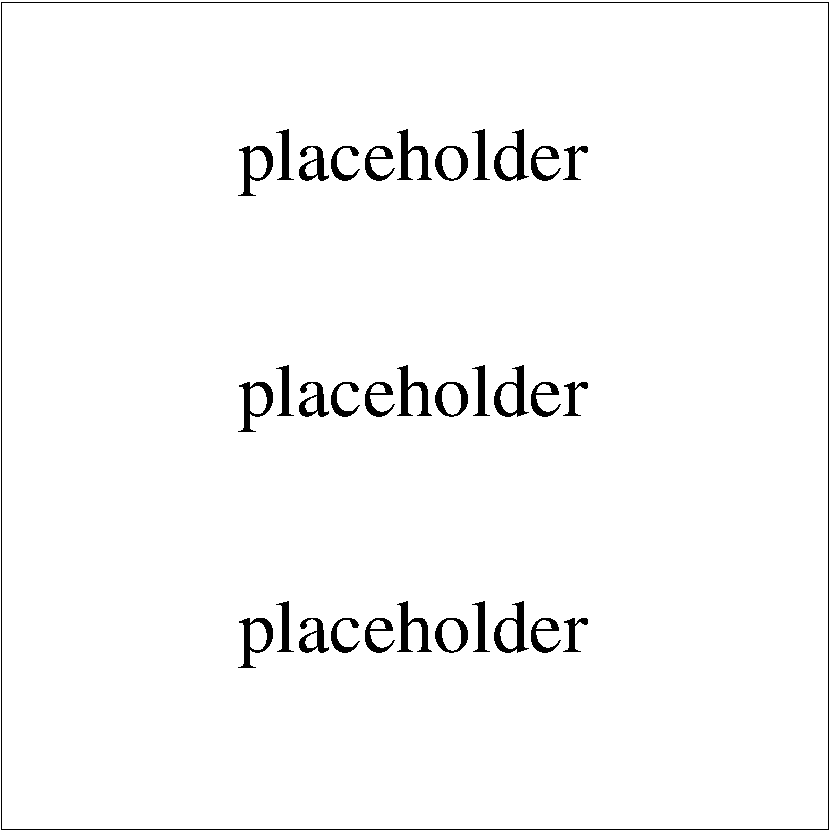
\includegraphics[width=2.5in]{evan/fig_evan_qdc_testing/placeholder.pdf}
\caption{A fixed-width integration gate, $T_{gate}$, and variable DC offsets, $V_1$-$V_7$ are used to calibrate the QDC, including sensitivity and pedestal measurements.\label{fig:qdcTest}}
\end{figure}

\begin{figure}[ht]
%\includegraphics[width=3.5in]{c_15_63_22_55mV.pdf}
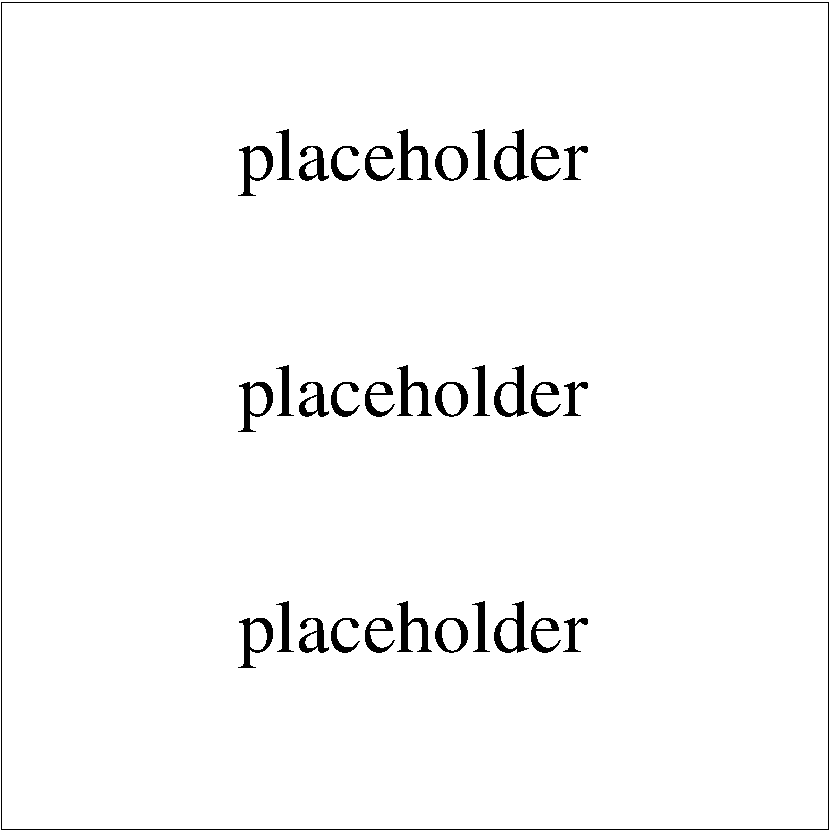
\includegraphics[width=3.5in]{evan/fig_evan_qdc_testing/placeholder.pdf}
\caption{An QDC distribution corresponding to a $-22.55\:mV$ offset integrated over $100\:ns$.\label{fig:QDCHist}}
\end{figure}

\begin{figure}
\centering
\mbox{\subfigure[$\:$DC offset versus QDC.]{
%\includegraphics[width=3.1in,height=2.8in]{c_15_63.pdf}\label{fig:offsetVQDC}
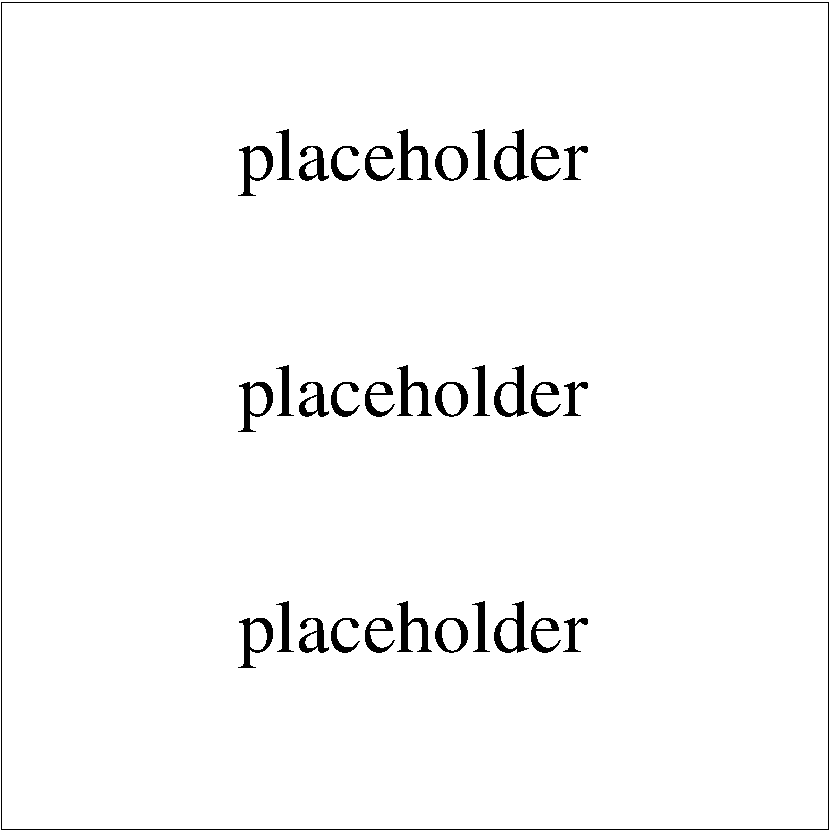
\includegraphics[width=3.1in,height=2.8in]{evan/fig_evan_qdc_testing/placeholder.pdf}\label{fig:offsetVQDC}
}\quad
\subfigure[$\:$Pedestal setting versus virtual ground.]{
%\includegraphics[width=3.1in,height=2.8in]{c_15.pdf}\label{fig:pedRange}
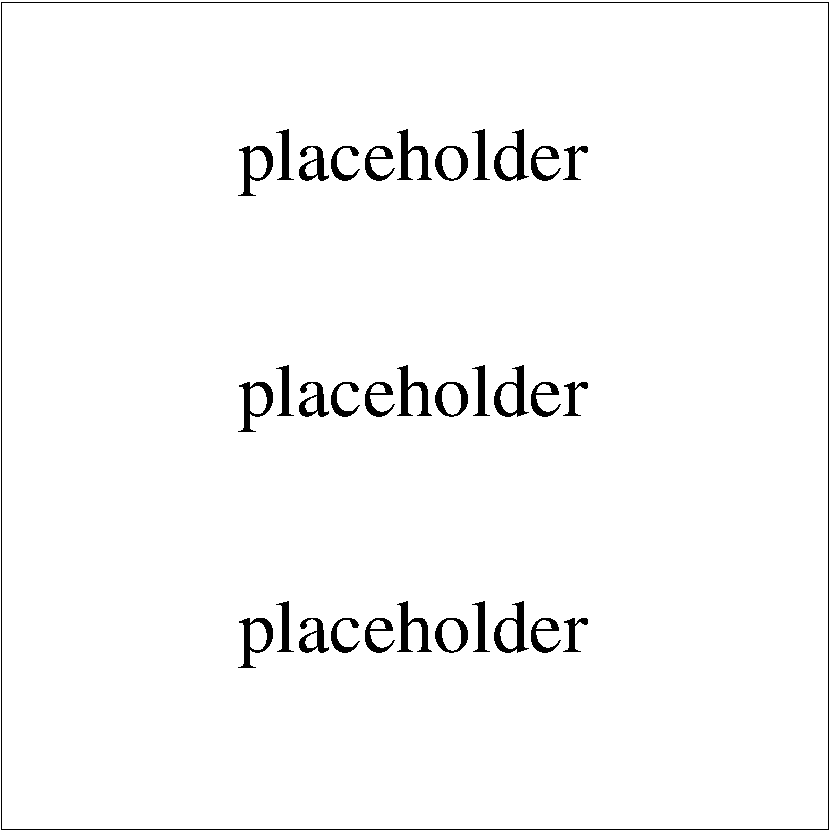
\includegraphics[width=3.1in,height=2.8in]{evan/fig_evan_qdc_testing/placeholder.pdf}\label{fig:pedRange}
}}
\caption{(a) For the adjustable pedestal setting of 63, the module has a virtual ground of $-4.6\:mV$ as determined by the QDC zero-crossing. (b) This zero-crossing varies from $\approx 0\:mV$ to $\approx -6\:mV$, so even in this case, an external DC offset is required to push the overall system offset into the active QDC range.}
\end{figure}

%\begin{figure}[ht]
%\includegraphics[width=5in]{c_15_63.pdf}
%\caption{\label{fig:offsetVQDC}}
%\end{figure}

%\begin{figure}[ht]
%\includegraphics[width=5in]{c_15.pdf}
%\caption{\label{fig:pedRange}}
%\end{figure}

Figure$\:$\ref{fig:QDCHist} illustrates the QDC distribution when the pedestal is set to 63 and an external DC offset of $-22.55\:mV$ is applied. Combining such results for various DC offsets, the relationship between the DC offset and QDC value is determined (see Fig.$\:$\ref{fig:offsetVQDC}). The $y$-intercept of the best-fit line indicates the QDC's virtual ground, its pedestal current, with respect to which it integrates incoming signals. Finally, the module's pedestal settings are compared to the corresponding virtual ground values to determine the full range of the adjustable intrinsic pedestal, as shown in Fig.$\:$\ref{fig:pedRange}.

The sensitivity of the QDC is determined from Fig.$\:$\ref{fig:offsetVQDC}, where the best-fit line is cast in terms of charge rather than DC offset as in equation \eqref{f:Q}, where $Q$ corresponds to total charge, $x$ to QDC value (bin), and $R$ to resistance ($50\:\Omega$).
\begin{equation}\label{f:Q}
Q=\left(-4.606\:\frac{mV}{bin}x - 0.0542\:mV\right)\left(\frac{T_{gate}}{R}\right) = -9.2\:\frac{pC}{bin}x - 0.11\:pC
\end{equation}
Accordingly, the V792N's sensitivity of $9.2\:\frac{pC}{bin}$ is consistent with the documented sensitivity of $10\:\frac{pC}{bin}$.
